\documentclass[10pt,mathserif]{beamer}
\usepackage[english]{babel}
\usepackage[utf8]{inputenc}
\usepackage[T1]{fontenc}
\usepackage{helvet}
\usepackage{nimbusmononarrow}
\usepackage{euler}
\usepackage{tikz}
\usepackage{listings}
\usepackage{relsize}
\usepackage{booktabs}

\usetikzlibrary{arrows}
\usetikzlibrary{backgrounds}
\usetikzlibrary{chains}
\usetikzlibrary{fit}
\usetikzlibrary{positioning}
\usetikzlibrary{scopes}
\usetikzlibrary{trees}
\usetikzlibrary{automata}
\usetikzlibrary{positioning}
\usetikzlibrary{shapes.multipart}

\usetheme{boxes}
%\useoutertheme{essential}
\usecolortheme{seagull}
\usefonttheme{structurebold}
\setbeamertemplate{navigation symbols}{}
\setbeamertemplate{frametitle}
{
	\begin{centering}
		\vspace{1.5em}
		\LARGE
    \insertframetitle
    \par
    \vspace{0.5em}
  \end{centering}
}
\setbeamerfont{title}{size=\huge}
\setbeamerfont{subtitle}{size=\Large}

\lstset{basicstyle=\ttfamily\scriptsize}
\newcommand{\cinput}[1]{\lstinputlisting[language=C,basicstyle=\ttfamily]{#1}}
\newcommand{\cinline}[1]{\lstinline[language=C,basicstyle=\ttfamily]!#1!}
\newcommand{\cppinput}[1]{\lstinputlisting[language=C++,basicstyle=\ttfamily]{#1}}
\newcommand{\cppinline}[1]{\lstinline[language=C++,basicstyle=\ttfamily]!#1!}
\newcommand{\llvminput}[1]{\lstinputlisting[language=LLVM,basicstyle=\ttfamily]{#1}}
\newcommand{\llvminline}[1]{\lstinline[language=LLVM,basicstyle=\ttfamily]!#1!}
\lstdefinelanguage{LLVM}%
  {morekeywords={define,declare,global,constant,internal,external,private,%
      linkonce,linkonce_odr,weak,weak_odr,appending,common,extern_weak,%
      thread_local,dllimport,dllexport,hidden,protected,default,except,deplibs,%
      volatile,fastcc,coldcc,cc,ccc,x86_stdcallcc,x86_fastcallcc,ptx_kernel,%
      ptx_device,signext,zeroext,inreg,sret,nounwind,noreturn,nocapture,byval,%
      nest,readnone,readonly,noalias,uwtable,inlinehint,noinline,alwaysinline,%
      optsize,ssp,sspreq,noredzone,noimplicitfloat,naked,alignstack,module,asm,%
      align,tail,to,addrspace,section,alias,sideeffect,c,gc,target,datalayout,%
      triple,blockaddress},%
  morekeywords=[2]{add,fadd,sub,fsub,mul,fmul,sdiv,udiv,fdiv,srem,urem,frem,%
     and,or,xor,icmp,fcmp,eq,ne,ugt,uge,ult,ule,sgt,sge,slt,sle,oeq,ogt,oge,%
     olt,ole,one,ord,ueq,ugt,uge,ult,ule,une,uno,nuw,nsw,exact,inbounds,phi,%
     call,select,shl,lshr,ashr,va_arg,trunc,zext,sext,fptrunc,fpext,fptoui,%
     fptosi,uitofp,sitofp,ptrtoint,inttoptr,bitcast,ret,br,indirectbr,switch,%
     invoke,unwind,unreachable,malloc,alloca,free,load,store,getelementptr,%
     extractelement,insertelement,shufflevector,extractvalue,insertvalue},%
  sensitive=t,%
  morestring=[b]",%
  morecomment=[l];%
  }[keywords,comments,strings]


\author{Daniele Cattaneo}
\institute{Politecnico di Milano}
\date{\DATE}
\title{Introduction to the LLVM compiler framework}
\subtitle{Welcome \& Course Outline}
\newcommand{\customdata}{Daniele Cattaneo <daniele.cattaneo@polimi.it>}

\AtBeginSection[]
{
\begin{frame}{Contents}
\tableofcontents[currentsection]
\end{frame}
}


\begin{document}

\begin{frame}
\maketitle
\end{frame}

\begin{frame}[plain]{}
  \begin{center}
    \vspace{-.1\textheight}
    
\includegraphics[width=\textwidth]{img/logo.png}
  \end{center}
\end{frame}
%--- Next Frame ---%

\begin{frame}[t]{About the dragon}
  \begin{itemize}
    \item The \textbf{LLVM logo} \cite{LOCAL:www/LLVMlogo} is a stylized
          wyvern (a kind of dragon). \\ \smallskip
          Dragons have connotations of power, speed and intelligence,
          and can also be sleek, elegant, and modular (err, maybe not).
    \pause
    \item There is a famous \textbf{compiler book} dating back to the 1970s
          with cover art featuring a knight fighting a dragon. 
          \cite{Aho:1977:PCD:1095594}
          \\ \smallskip After all, compilers are also \textbf{scary}...
  \end{itemize}
  \begin{center}
    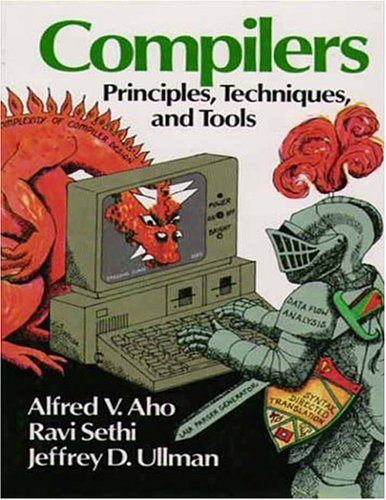
\includegraphics[height=.3\paperheight]{img/red_dragon_book.jpg}
    \hspace{2em}
    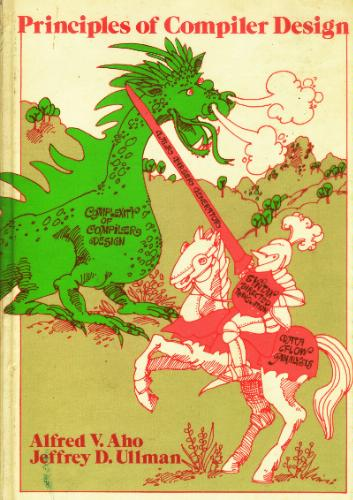
\includegraphics[height=.3\paperheight]{img/green_dragon_book.jpg}
    \hspace{2em}
    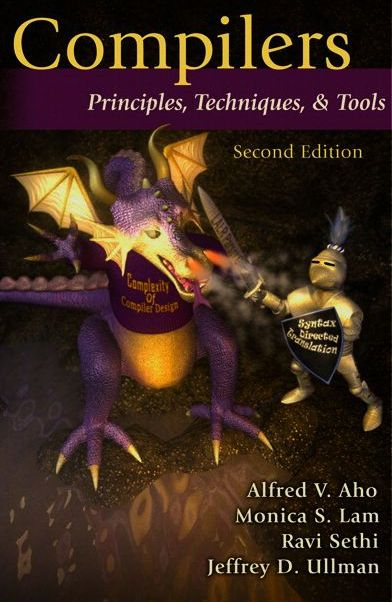
\includegraphics[height=.3\paperheight]{img/purple_dragon_book.jpg}
  \end{center}
\end{frame}
%--- Next Frame ---%

\begin{frame}[t]{About LLVM}
  \begin{center}
  	\vfill
  	\large
  	The idea behind LLVM is that \\ compilers should \textbf{NOT} be scary! \\
		\bigskip
		Instead, they should be \textbf{easy} \\ to extend and hack at your leisure. \\
		\bigskip
		In this course we will see how to have fun with compilers, \\instead of being scared of them.
		\vfill
  \end{center}
\end{frame}
%--- Next Frame ---%

\begin{frame}[t]{About me}
	\vspace{\stretch{1}}
  \begin{large}
  \begin{center}
    Daniele Cattaneo
  \end{center}
  \end{large}
  \vspace{0.5em}
  \begin{center}
  \begin{varwidth}{8cm}
    \begin{itemize}
    \item \texttt{daniele.cattaneo@polimi.it}
    \item PhD candidate @ Politecnico di Milano (Italy)
    \item Obsessed with compilers for a long time...
    \item ...now working on research projects with LLVM!
    \item (yes I have strange tastes, I know)
  \end{itemize}
  \end{varwidth}
  \end{center}
  \vspace{\stretch{3}}
\end{frame}
%--- Next Frame ---%

\begin{frame}[t]{About you}
	\vspace{\fill}
	\begin{center}
  \begin{varwidth}{8.5cm}
  In order to fully understand the content of this course,
  you should have:
  \smallskip
  \begin{itemize}
    \item knowledge of what a compiler is
    \item proficiency in the most common data structures
    \item proficiency in Object-Oriented Programming
    \item at least some experience with C++
  \end{itemize}
  \end{varwidth}
  \medskip
  \end{center}
   \begin{center}
  \textbf{\large That's it!}
  \end{center}
  \vspace{\fill}
\end{frame}
%--- Next Frame ---%

\begin{frame}[t]{About the course}
\begin{center}
\begin{varwidth}{8.5cm}
  \begin{Large}
  \begin{enumerate}
  	\setlength\itemsep{8pt}
    \item First part \vspace{6pt}
      \begin{itemize}
      	\normalsize \setlength\itemsep{4pt}
        \item Compiler design
        \item LLVM structure overview
        \item LLVM-IR language
    	\end{itemize}
    \item Second part \vspace{6pt}
      \begin{itemize}
      \normalsize \setlength\itemsep{4pt}
        \item LLVM Documentation
        \item Available middle-end passes (overview)
        \begin{itemize}
        	\normalsize
          \item Normalization
          \item Analysis
        \end{itemize}
        \item LLVM quick start tutorial (depending on time)
      \end{itemize}
  \end{enumerate}
	\end{Large}
\end{varwidth}
\end{center}
\end{frame}
%--- Next Frame ---%

\begin{frame}[t]{Goal of the course}
	\vspace{\stretch{1}}
	\begin{center}
	\begin{varwidth}{8.5cm}
  At the end of these lectures you will (hopefully)\\ be able to:
  \medskip
  \begin{itemize}
    \item understand the LLVM compiler infrastructure
    \item read a .ll file (LLVM-IR)
    \item know where to look for documentation
    \item know which middle-end weapons
          LLVM provides you, out of the box
    \item know how to implement a simple analysis / transformation
    \item know how to test your code
  \end{itemize}
  \end{varwidth}
  \end{center}
  \vspace{\stretch{3}}
\end{frame}
%--- Next Frame ---%

\section*{Bibliography}
\begin{frame}[allowframebreaks]{Bibliography}
\nocite{*}
\bibliographystyle{unsrt}
\bibliography{bibliography-0}
\end{frame}

\end{document}
